\section{Actors}
\label{sec:actors}

\begin{figure}[t]
  \label{fig:actors}
  \caption{Actors of the system}
  \begin{center}
    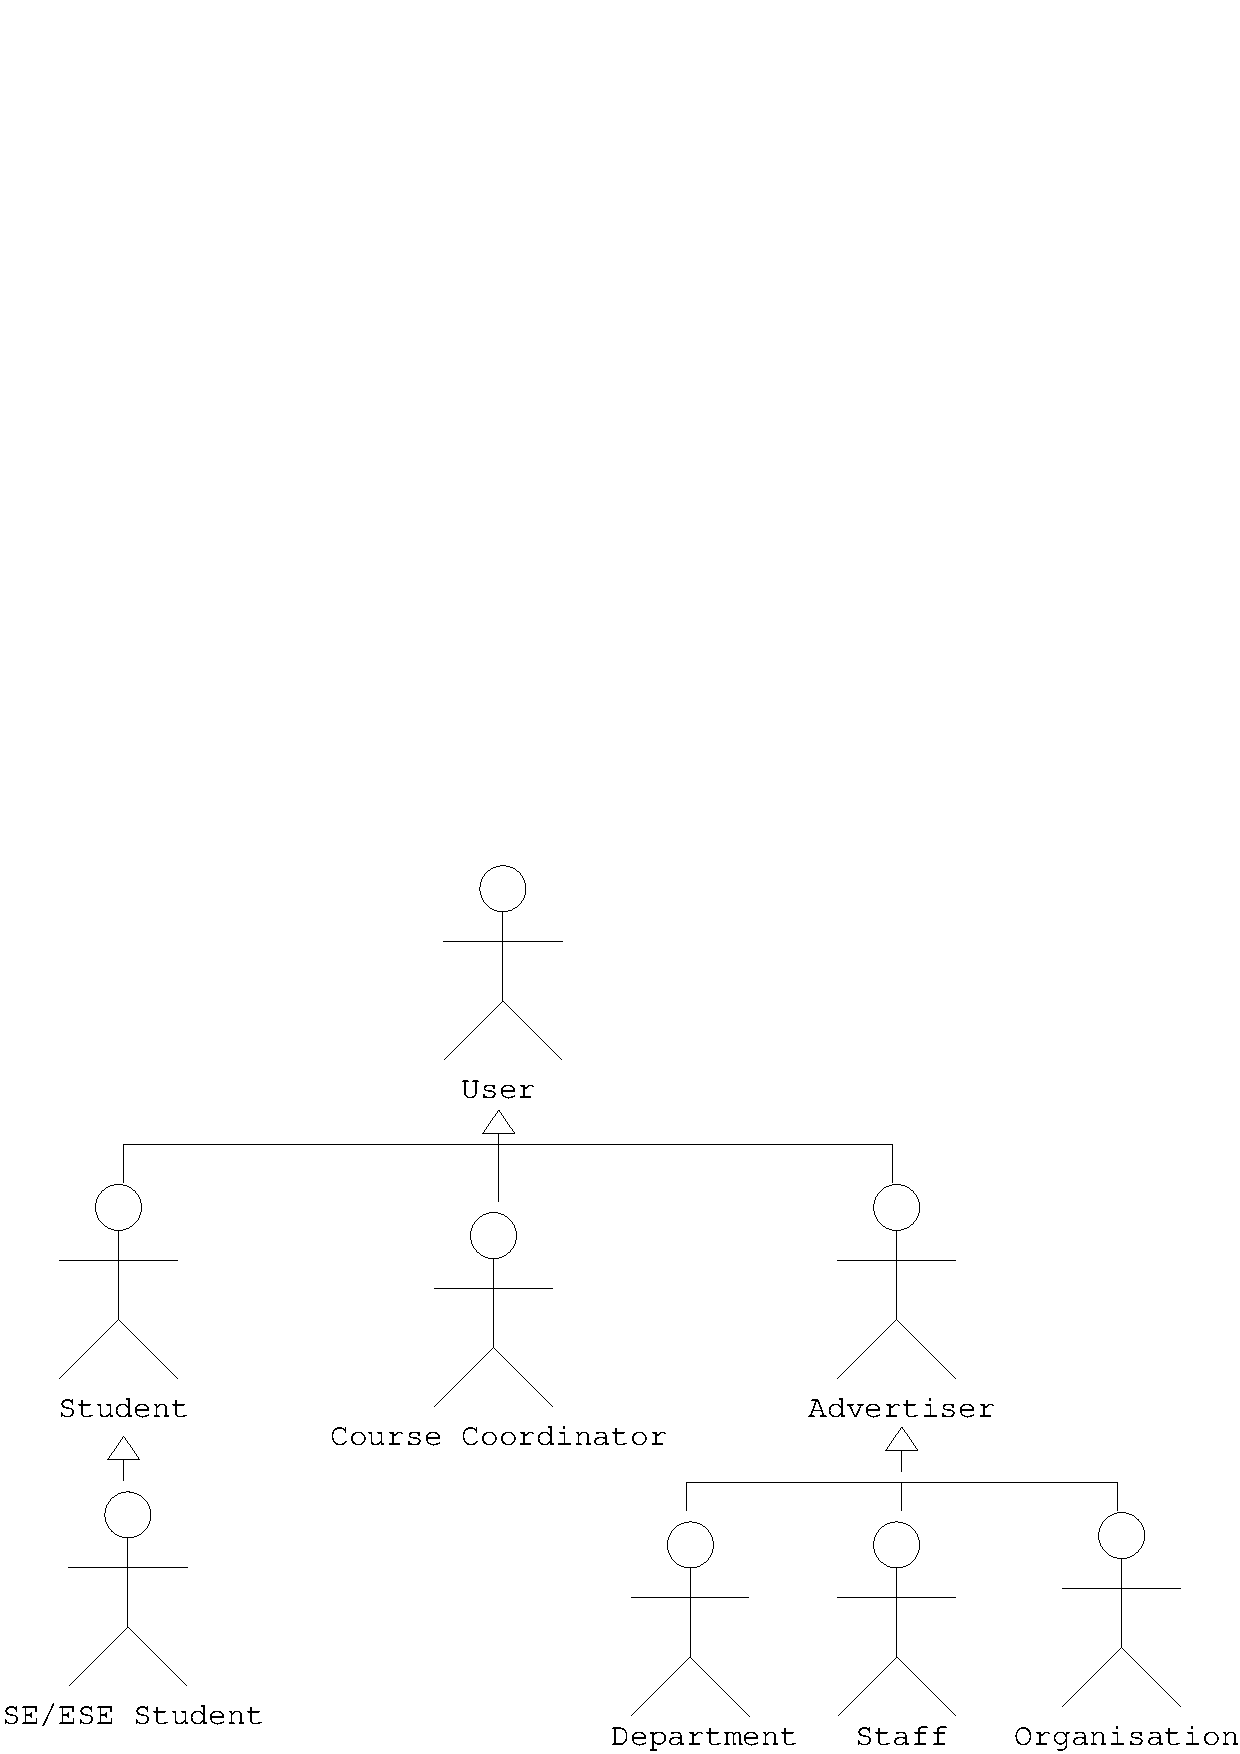
\includegraphics[width=0.9\textwidth]{img/actors.pdf}
  \end{center}
\end{figure}

Figure \ref{fig:actors} illustrates the relationships between actor roles in the system.
A short summary of the actors is given below:

\begin{description}
\item[User]{A user of the system}
\item[Advertiser] {A user who can advertise internships}
\item[Organisation] {An advertiser belonging to an organisation outwith the University}
\item[Academic] {An advertiser who is an academic at the University}
\item[Student] {A user who is a Computing Science student at the University}
\item[SE/ESE Student] {A student studying Software Engineering or Electronics and Software Engineering}
\item[Staff] {A user who is a member of staff at the University}
\item[Course Coordinator] {A type of Staff who acts as the bridge between Advertisers and Students}
\end{description}

\section{Use Cases}
\label{sec:usecases}

This section describes the required functionality for the Internship Management System as \textbf{X} groups of related use cases. 
The core use cases for the system are:

\begin{itemize}
  \item{Common Utilities (Section \textbf{X})}
    \begin{itemize}
      \item{Search for Advert}
      \item{Search for User}
      \item{\ldots}
    \end{itemize}
  \item{Submitting Advertisements (Section X)}
    \begin{itemize}
    \item{Submit advertisement for review}
    \item{Review advertisement}
    \item{Comment advertisement}
    \item{Publish advertisement}
    \end{itemize}
\end{itemize}
